\documentclass[17pt]{beamer}
\usepackage[T1]{fontenc}
\usepackage[utf8]{inputenc}
\usepackage{graphicx}
\usetheme{Madrid}
\usecolortheme{beaver}
 
%Information to be included in the title page:
\title{Wprowadzenie do Pythona}
\subtitle{Część 1/2}
\author{Tomasz Derek}
\institute{KMS}
\date{Październik 16, 2019}
 
\begin{document}
 
\frame{\titlepage}
 
\begin{frame}
\frametitle{Dlaczego Python?}
\begin{itemize}
\item Wpisać mądre zdanie
\end{itemize}
\end{frame} 
 
\begin{frame}
\frametitle{Plusy Pythona}
\begin{itemize}
\item Prostota języka
\item Wiele zastosowań
\item Automatyczne zarządzanie pamięcią
\item Łatwość tworzenia kodu
\item Powszechnie używany w AI
\end{itemize}
\end{frame}

\begin{frame}
\frametitle{Plusy Pythona}
\begin{figure}[ht]

\includegraphics[scale=0.25]{./kiddo.jpeg}
\end{figure}
\end{frame}

\begin{frame}
\frametitle{Minusy Pythona}
\begin{itemize}
\item Wydajność
\item GIL
\item Rozbicie na wersję 2 i 3
\item Tworzenie GUI
\end{itemize}
\end{frame}

\begin{frame}
\frametitle{Minusy Pythona}
\begin{figure}[ht]

\includegraphics[scale=0.3]{./war.jpeg}
\end{figure}
\end{frame}

\begin{frame}
\frametitle{Z czego będziemy korzystać?}
\begin{figure}[ht]
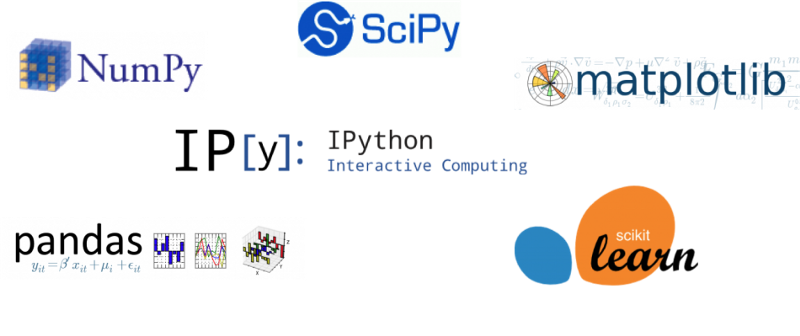
\includegraphics[scale=0.3]{./modules.png}
\end{figure}
\end{frame}

\begin{frame}
\frametitle{Z czego będziemy korzystać?}
\begin{figure}[ht]
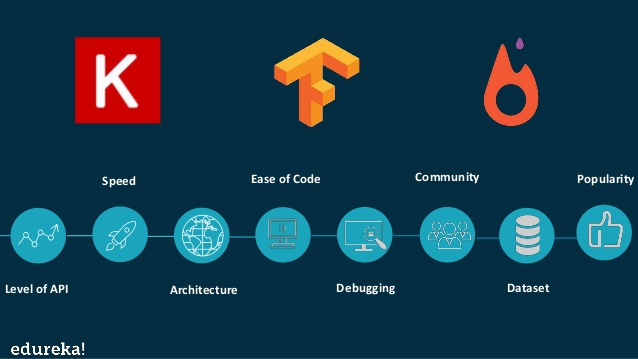
\includegraphics[scale=0.3]{./frameworks.jpg}
\end{figure}
\end{frame}

\end{document}https://github.com/HyperScypion/KMS_Neural_Networks/tree/master/lectures/second_lecture/notebooks